\section{The Ising model}


\begin{figure}[H]
  \begin{center}
    \includegraphics[width=0.95\textwidth]{Figures/Plots/Ising/Result14conv}
  \end{center}
  \caption{The convergence graph of the RBM mean energy output for the Ising model with $N = 14$ particles, $M=1$, and $J=-1$ and $L=-0.5$.}
\end{figure}

The two-dimensional Ising model results in the following convergence graph:

\begin{figure}[H]
  \begin{center}
    \includegraphics[width=0.95\textwidth]{Figures/Plots/Ising/Result9conv}
  \end{center}
  \caption{The convergence graph of the RBM mean energy output for the two-dimensional Ising model with $N = 3$ particles, $M=3$, and $J=-1$ and $L=-0.5$.}
\end{figure}

\subsection{The effect of \texorpdfstring{$J$}{J} on RBM prediction accuracy}

\begin{figure}[H]
  \begin{center}
    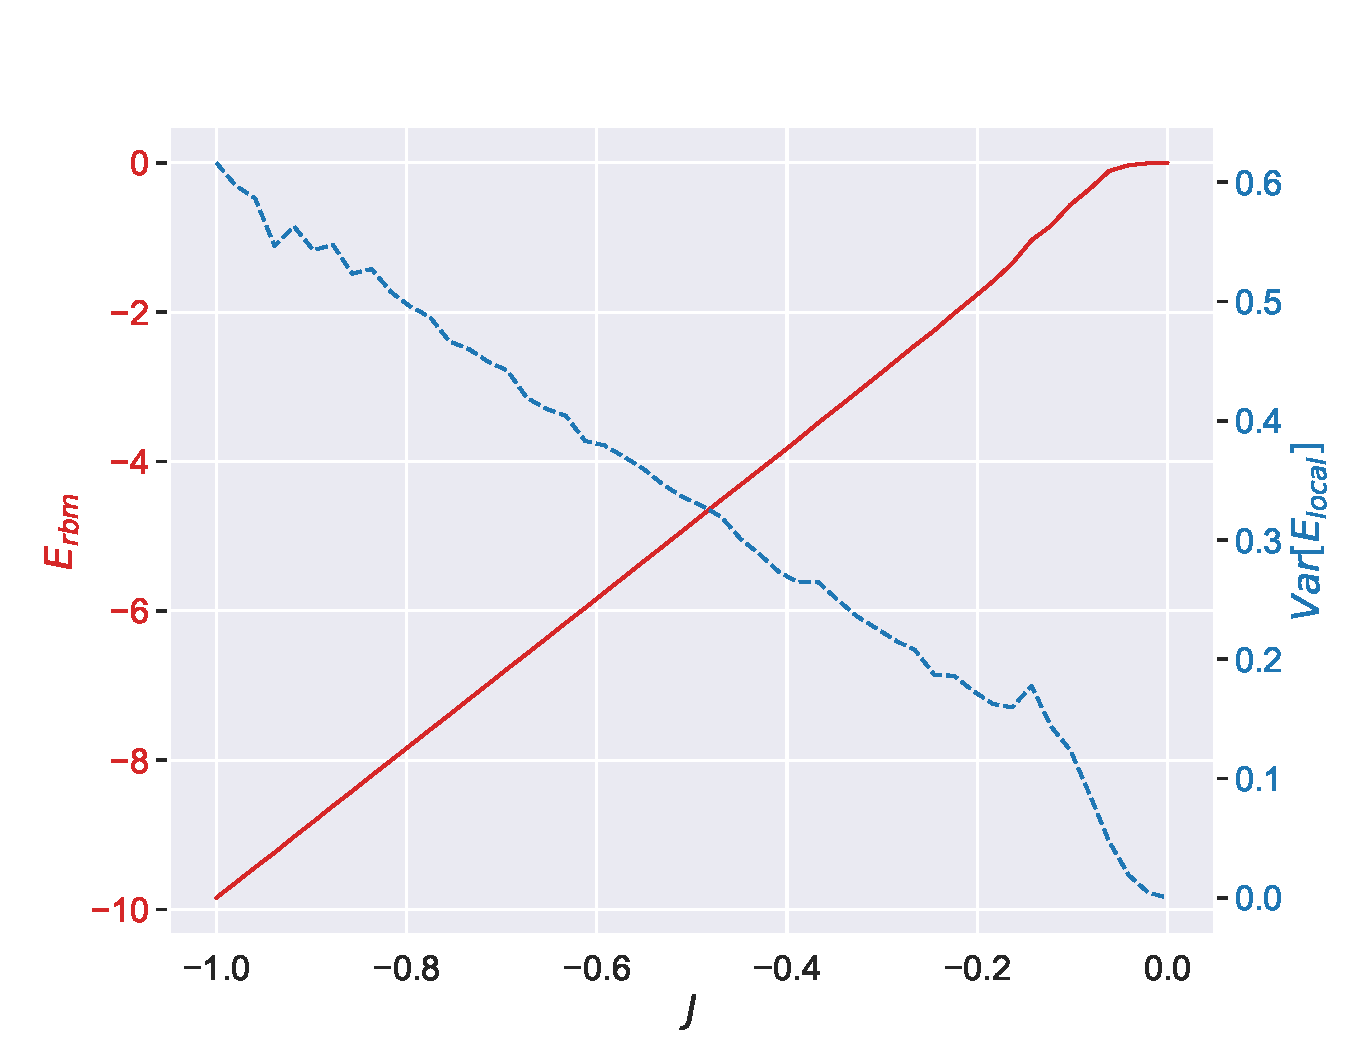
\includegraphics[width=0.95\textwidth]{Figures/Plots/Ising/[J][-1.0-0.0][e=500][n=10][L=0]}
  \end{center}
  \caption{The variance of the restricted Boltzmann machine local energy output for the Ising model with $10$ lattice points and $L=0$.}
\end{figure}


\begin{figure}[H]
  \begin{center}
    \includegraphics[width=0.95\textwidth]{Figures/Plots/Ising/[J][-1.0-0.0][e=500][n=10][L=-0.5]}
  \end{center}
  \caption{The variance of the restricted Boltzmann machine local energy output for the Ising model with $10$ lattice points and $L=-0.5$.}
\end{figure}

Looking at the two-dimensional version we get

\begin{figure}[H]
  \begin{center}
    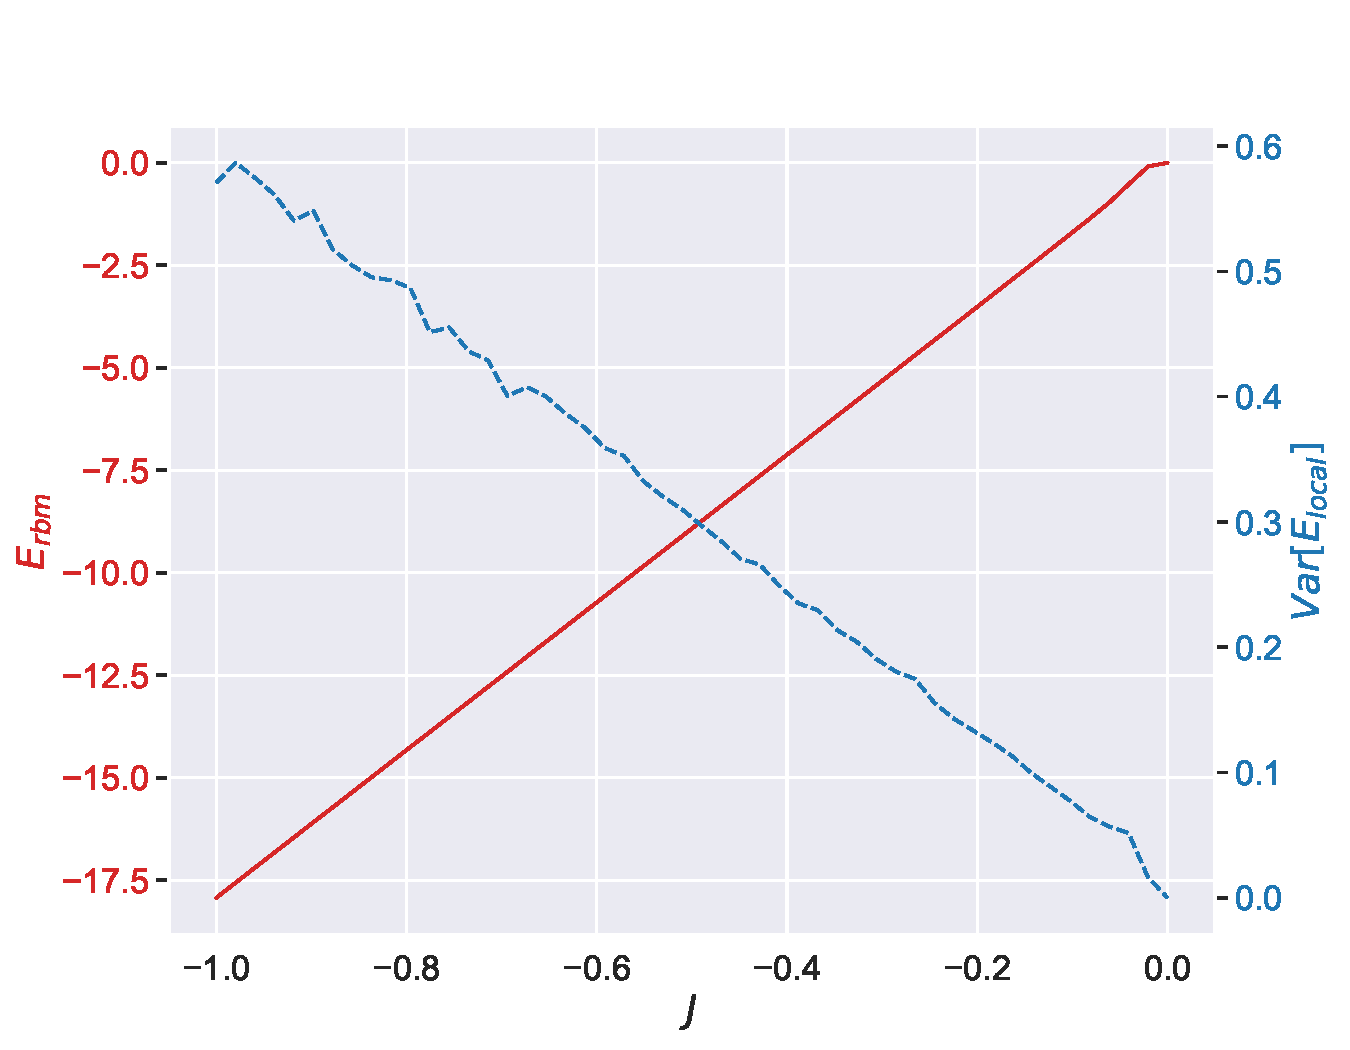
\includegraphics[width=0.95\textwidth]{Figures/Plots/Ising/[J][-1.0-0.0][e=500][n=9][L=0]}
  \end{center}
  \caption{The variance of the restricted Boltzmann machine local energy output for the two=two-dimensional Ising model with $9$ lattice points, $N=3$ and $M=3$, and $L=0$.}
\end{figure}


\begin{figure}[H]
  \begin{center}
    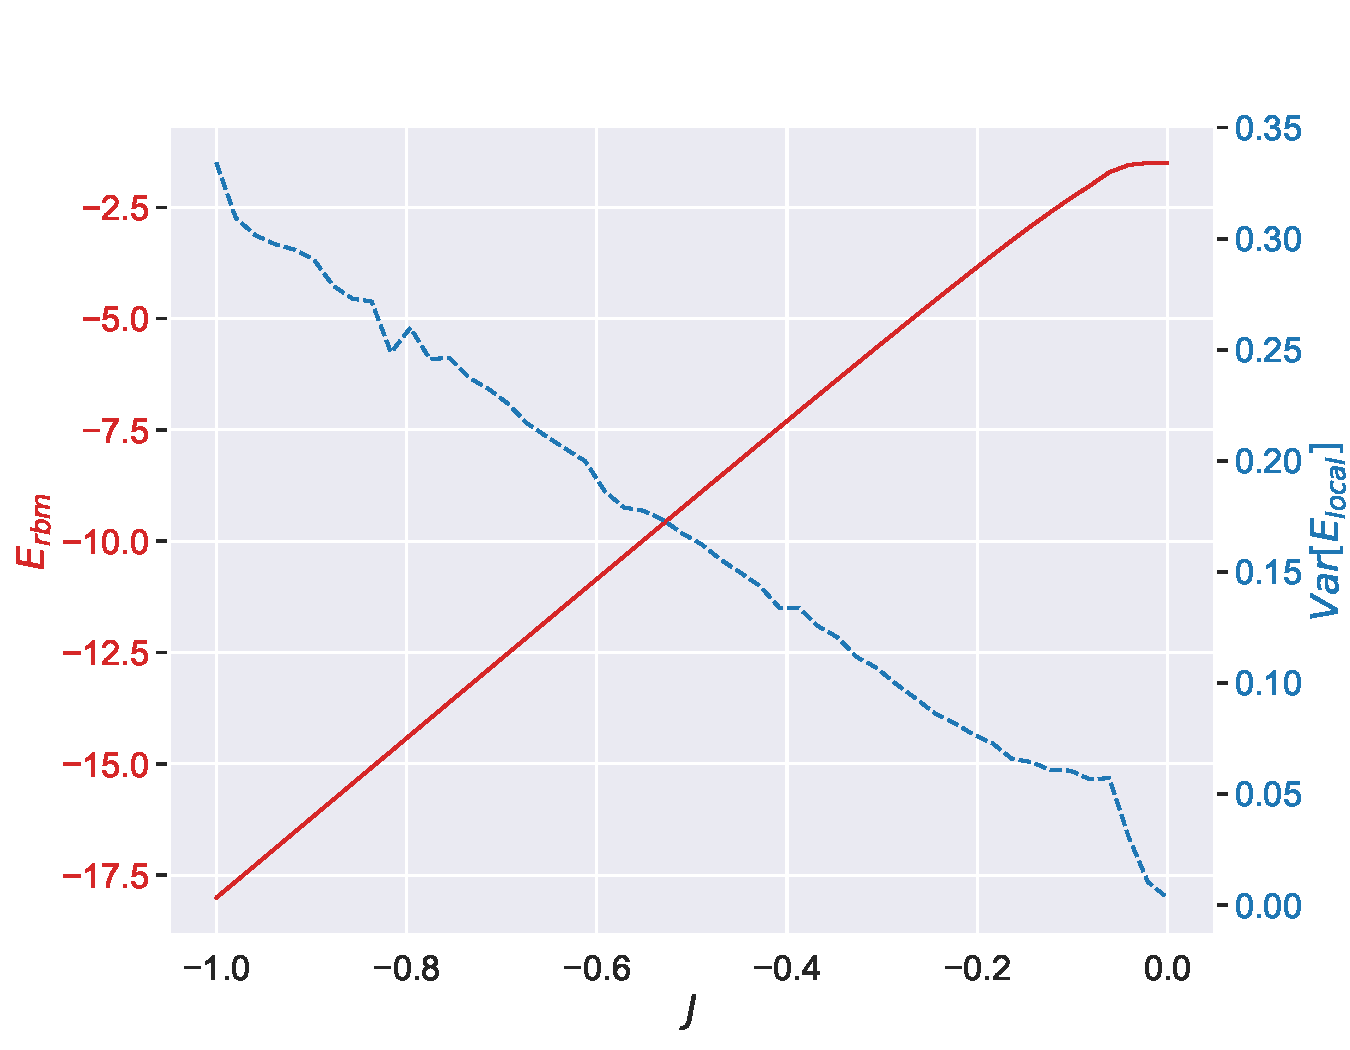
\includegraphics[width=0.95\textwidth]{Figures/Plots/Ising/[J][-1.0-0.0][e=500][n=9][L=-0.5]}
  \end{center}
  \caption{The variance of the restricted Boltzmann machine local energy output for the two-dimensional Ising model with $9$ lattice points, $N=3$ and $M=3$, and $L=-0.5$.}
\end{figure}
\subsection{The effect of \texorpdfstring{$L$}{L} on RBM prediction accuracy}

\begin{figure}[H]
  \begin{center}
    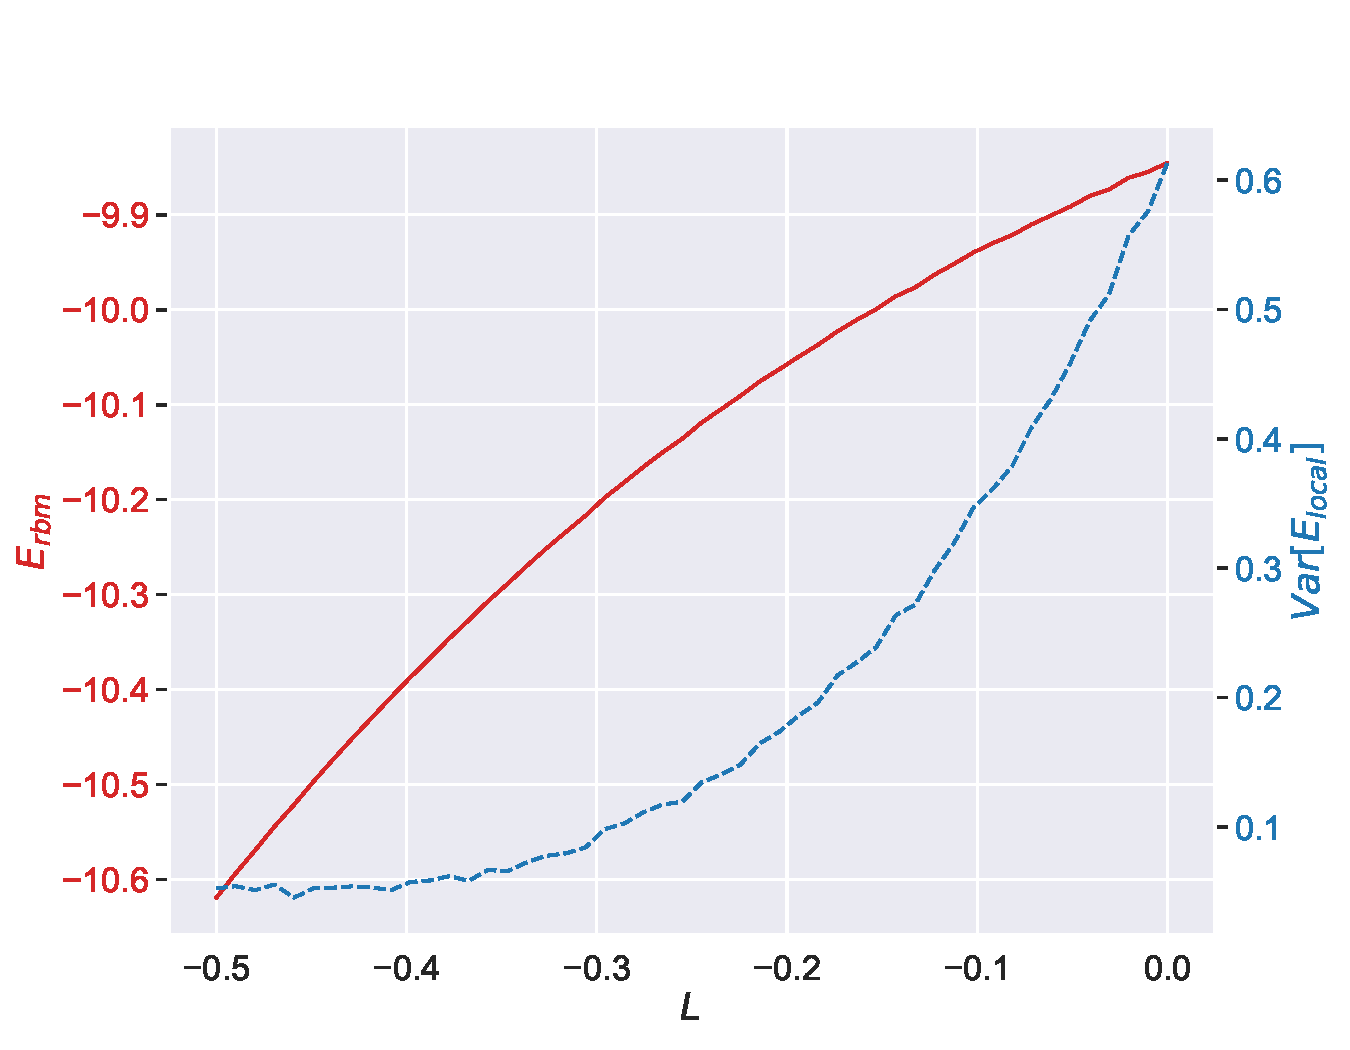
\includegraphics[width=0.95\textwidth]{Figures/Plots/Ising/[L][-0.5-0.0][e=500][n=10][J=-1]}
  \end{center}
  \caption{The variance of the restricted Boltzmann machine local energy output for the Ising model with $10$ lattice points and $J=-1$.}
\end{figure}

And with two dimensions

\begin{figure}[H]
  \begin{center}
    \includegraphics[width=0.95\textwidth]{Figures/Plots/Ising/[L][-0.5-0.0][e=500][n=9][J=-1]}
  \end{center}
  \caption{The variance of the restricted Boltzmann machine local energy output for the Ising model with $9$ lattice points, $N=3$ and $M=3$, and $J=-1$.}
\end{figure}

\subsection{Comparing computation time with diagonalization}
